\documentclass[11pt]{article}

\def\mainroot{ell_1}

\usepackage[top=1in, bottom=1in, left=1in, right=1in]{geometry}

\usepackage[compact]{titlesec}

\usepackage{xcolor}
\definecolor{pykeyword}{HTML}{000088}
\definecolor{pyidentifier}{HTML}{000000}
\definecolor{pystring}{HTML}{008800}
\definecolor{pynumber}{HTML}{FF4000}
\definecolor{pycomment}{HTML}{880000}

\usepackage{listings}
\lstset{language=Python,
	basicstyle=\ttfamily\small,
	tabsize=4,
	showstringspaces=false,
	keywordstyle=\color{pykeyword},
	identifierstyle=\color{pyidentifier},
	stringstyle=\color{pystring},
	numberstyle=\color{pynumber},
	commentstyle=\color{pycomment}
}

\usepackage{algorithm}
\usepackage{algpseudocode}

\usepackage{graphicx}

\usepackage{amsmath}
\usepackage{enumitem}

\title{CSE 537 Assignment 5 Report: ML Classifiers}

\author{
Remy Oukaour \\
	{\small SBU ID: 107122849}\\
	{\small \texttt{remy.oukaour@gmail.com}}
\and
Jian Yang \\
	{\small SBU ID: 110168771}\\
	{\small \texttt{jian.yang.1@stonybrook.edu}}
}

\date{Wednesday, December 9, 2015}

\raggedbottom

\begin{document}

\maketitle

\section{Introduction}

This report describes our submission for assignment 5 in the CSE 537 course on
artificial intelligence. Assignment 5 requires us to implement two kinds of
machine learning classifiers: a decision tree classifier for predicting credit
worthiness of applicants, and a na{\"i}ve Bayes classifier for classifying
handwritten digits. In this report, we discuss the implementation details and
performance of our solutions.

\section{Decision tree classifier}

Jian Yang developed the decision tree classifier for predicting credit worthiness
of applicants.

% TODO

\section{Na{\"i}ve Bayes classifier}

Remy Oukaour developed the na{\"i}ve Bayes classifier for classifying handwritten
digits.

\subsection{Instructions}

To run the classifier, enter $python\ naive\text{-}bayes.py$. It will read from
$trainingimages.txt$, $traininglabels.txt$, $testimages.txt$, and $testlabels.txt$,
and output to $predictedlabels.txt$ and $confusion\text{-}matrix.txt$.

\subsection{Implementation}

The classifier is a straightforward implementation of na{\"i}ve Bayes, using the formula
``log posterior $\propto$ log prior + log likelihood'':

$$\log P(label|features) \propto \log P(label) + \sum_{feature} P(feature|label)$$

The prior probability $P(label)$ is estimated to be the fraction of training instances
with a given label (0 to 9). The likelihood $P(feature|label)$ of a feature having a
certain value for a test instance is estimated to be the fraction of training instances
(limited to that label) with that value for that feature. (We use Laplace smoothing to
handle novel feature values in the test data, with a smoothing value of 0.001.) We then
pick the label of each test instance using a maximum likelihood estimator:

$$classification(features) = \underset{labels}{\operatorname{argmax}} \ \log P(label|features)$$

\subsection{Feature selection}

We tested many different kinds of features to maximize performance. First, we decided
how to use the images' pixel values: whether to treat gray as black, and whether to use
groups of pixels as individual features. We counted the number of correctly classified
test instances for each alternative.

\begin{itemize}[noitemsep]
\item Individual pixels: 772 correct
\item 2$\times$2 blocks: 849 correct
\item 2$\times$2 overlapping blocks: 861 correct
\item 3$\times$3 blocks, 1-overlapping: 819 correct
\item 3$\times$3 blocks, 2-overlapping: 821 correct
\item 4$\times$4 blocks: 689 correct
\item 4$\times$4 blocks, 1-overlapping: 725 correct
\item 4$\times$4 blocks, 2-overlapping: 742 correct
\item 4$\times$4 blocks, 3-overlapping: 758 correct
\end{itemize}

We chose to use 2$\times$2 overlapping blocks of pixels as features.

We also tried treating gray pixels (``+'') as black ones (``\#''), but this lowered
accuracy from 861 to 857 correct.

The Laplace smoothing value of 0.001 was likewise chosen via testing. We expected 1 to
work well, but it did not improve the accuracy from 861. Higher values actually lowered
the accuracy, so we tried lower values until they no longer provided more benefit. With
smoothing of 0.001, we reached 893 correctly classified test instances.

At this point we added an minimum entropy threshold for the features, on the grounds
that a low-entropy feature would just be adding noise. (Many pixel-block features around
the edges of the digit images are completely white for all training and test images,
thus having 0 entropy and providing no benefit.) Testing a range of threshold values from
0 to 0.3, we found a peak at 0.15, with 897 correct classifications.

To achieve at least 90\% accuracy, we added holistic features:

\begin{itemize}[noitemsep]
\item $num\_regions$: a count of contiguous regions in the image, treating gray and black
pixels as ``foreground'' and white as ``background,'' counted using a flood-fill algorithm.
\item $spread\_ratio$: the ratio of vertical to horizontal foreground ``spread.'' Spread
is the total distance of all foreground pixels from a center line.
\item $horizontal\_bias$: the difference between the number of foreground pixels in the
top and bottom halves of the image.
\item $vertical\_bias$: the difference between the number of foreground pixels in the
left and right halves of the image.
\end{itemize}

By adding these features to the existing block-based ones, we were able to correctly
classify 903 out of 1,000 test instances.

\subsection{Performance results}

The classifier's precision for all ten digits ranged from 79.5\% (for 8) to 96.3\% (for 1).
The sensitivity ranged from 81.1\% (for 7) to 95.6\% (for 0). The overall accuracy was 90.3\%.

\begin{table}[h!]
\centering
\setlength\tabcolsep{4pt}
\begin{tabular}{| r | r | r | r | r | r | r | r | r | r | r | r | r |}
\hline
\textbf{pred\textbackslash true} & \textbf{0} & \textbf{1} & \textbf{2} & \textbf{3} & \textbf{4} & \textbf{5} & \textbf{6} & \textbf{7} & \textbf{8} & \textbf{9} & \textbf{total} & \textbf{precision} \\
\hline
\textbf{0} & 86 & 0 & 1 & 0 & 0 & 1 & 1 & 0 & 1 & 1 & 91 & 94.5\% \\
\hline
\textbf{1} & 0 & 103 & 0 & 0 & 0 & 0 & 1 & 3 & 0 & 0 & 107 & 96.3\% \\
\hline
\textbf{2} & 0 & 1 & 95 & 2 & 0 & 1 & 0 & 5 & 2 & 0 & 106 & 89.6\% \\
\hline
\textbf{3} & 0 & 0 & 1 & 91 & 0 & 2 & 0 & 0 & 7 & 2 & 103 & 88.3\% \\
\hline
\textbf{4} & 0 & 1 & 0 & 0 & 101 & 0 & 0 & 0 & 2 & 3 & 107 & 94.4\% \\
\hline
\textbf{5} & 0 & 0 & 0 & 3 & 0 & 81 & 4 & 1 & 1 & 1 & 91 & 89.0\% \\
\hline
\textbf{6} & 1 & 1 & 1 & 0 & 2 & 0 & 83 & 0 & 0 & 0 & 88 & 94.3\% \\
\hline
\textbf{7} & 1 & 0 & 1 & 1 & 1 & 0 & 0 & 86 & 1 & 1 & 92 & 93.5\% \\
\hline
\textbf{8} & 2 & 2 & 4 & 1 & 0 & 6 & 2 & 2 & 89 & 4 & 112 & 79.5\% \\
\hline
\textbf{9} & 0 & 0 & 0 & 2 & 3 & 1 & 0 & 9 & 0 & 88 & 103 & 85.4\% \\
\hline
\textbf{total} & 90 & 108 & 103 & 100 & 107 & 92 & 91 & 106 & 103 & 100 & 1000 & \\
\hline
\textbf{sensitivity} & 95.6\% & 95.4\% & 92.2\% & 91.0\% & 94.4\% & 88.0\% & 91.2\% & 81.1\% & 86.4\% & 88.0\% & & \\
\hline
\end{tabular}
\caption{Confusion matrix with precision and sensitivity scores for all ten labels.}
\label{nbc_confusion_matix}
\end{table}

The most common errors were to misclassify a 7 as a 9 (which happened 9 times), an 8 as
a 3 (which happened 7 times), or a 5 as an 8 (which happened 6 times). These are all the
kind of errors that a human judge could also make with sloppy handwriting. In addition,
of the 97 misclassified digits, some are illegible even for humans.

\begin{figure}[h!]
\centering
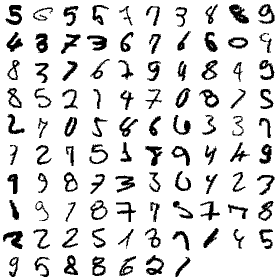
\includegraphics[height=2.75in, width=2.75in]{digits.png}
\caption{The 97 digits which the na{\"i}ve Bayes classifier got wrong.}
\label{nbc_digits}
\end{figure}

\end{document}
